\documentclass{standalone}

\usepackage{tikz}
\usetikzlibrary{positioning}
\usetikzlibrary{calc} % Only for Imagemagick workaround

\begin{document}

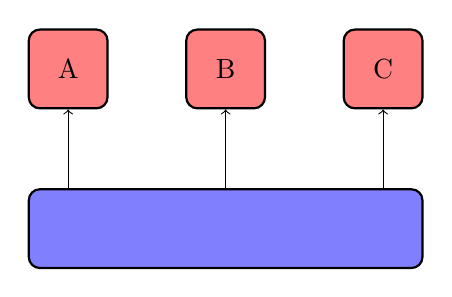
\begin{tikzpicture}[
  every node/.style={draw, minimum size=1cm, thick, fill=white, rounded corners},
  hi/.style={fill=red!50},
  low/.style={fill=blue!50},
]
  \node[low, minimum width=5cm] (basis) {};
  \node[hi, above=of basis.north west, anchor=south west] (a) {A};
  \node[hi, above=of basis] (b) {B};
  \node[hi, above=of basis.north east, anchor=south east] (c) {C};

  \draw[->] (basis.north -| a) -- (a);
  \draw[->] (basis) -- (b);
  \draw[->] (basis.north -| c) -- (c);

  % Workaround for Imagemagick `convert' cropping top pixels
  \useasboundingbox (current bounding box.south west) rectangle ($(current bounding box.north east) + (0, 0.01)$);
\end{tikzpicture}

\end{document}
